\documentclass[aps,pra,superscriptaddress,notitlepage,twocolumn]{revtex4-1}
\usepackage{amsmath,amssymb}
\usepackage[utf8x]{inputenc}
\usepackage[english]{babel}
\usepackage{graphicx,epsfig}
%\usepackage{txfonts}
\usepackage{xspace}
\usepackage[colorlinks=true,linkcolor=blue,urlcolor=blue,citecolor=blue]{hyperref}
\usepackage{dsfont}
\usepackage{stmaryrd}
\usepackage[usenames,dvipsnames]{color}
\usepackage[normalem]{ulem}
\usepackage{todonotes}


\bibliographystyle{apsrev4-1}
%%%%%%% commands %%%%%%%%%%%%

\newcommand{\ys}[1]{\todo[inline,backgroundcolor=purple!20!white]{\textcolor{Black}{{\bf Yulia:} #1}}}
\newcommand{\kis}[1]{\todo[inline,backgroundcolor=orange!20!white]{\textcolor{Black}{{\bf Kushal:} #1}}}
\newcommand{\todoall}[1]{\todo[inline,backgroundcolor=orange!20!white]{\textcolor{Black}{{\bf Yulia and Kushal:} #1}}}


\newcommand{\edit}[1]{{\color{blue}{#1}}}    % Uncomment if you want to see editing as blue
%\newcommand{\todo}[1]{{\color{red}{\textbf{ToDo: #1}}}}
% \newcommand{\ys}[1]{{\color{cyan}{#1}}}  
% \newcommand{\kis}[1]{{\color{dgreen}{#1}}}  

\definecolor{dgreen}{rgb}{0.0, 0.5, 0.0}
\newcommand{\rcomment}[1]{\textcolor{dgreen}{[RS: {#1}]}}

\newcommand{\vecr}{\mathbf r}
\newcommand{\veck}{\mathbf k}
\newcommand{\vecp}{\mathbf p}
\newcommand{\vecq}{\mathbf q}
\newcommand{\bed}{\hat b^\dag }
\newcommand{\be}{\hat b }


\definecolor{dgreen}{rgb}{0.0, 0.5, 0.0}
\newcommand{\gtext}[1]{\textcolor{dgreen}{[#1]}}

\newcommand{\comment}[1]{\textbf{[{#1}]}}
\newcommand{\bcomment}[1]{\textcolor{blue}{\textbf{[{#1}]}}}
\newcommand{\rtext}[1]{\textcolor{red}{{#1}}}
\newcommand{\btext}[1]{\textcolor{blue}{{#1}}}
\newcommand{\vtext}[1]{\textcolor{violet}{{#1}}}
\newcommand{\oldtext}[1]{\textcolor{red}{\sout{#1}}}
\definecolor{dgreen}{rgb}{0.0, 0.5, 0.0}
\newcommand{\fcomment}[1]{\footnote{{\textcolor{dgreen}{{#1}}}}}

\renewcommand{\vec}{\mathbf}


\newcommand{\vecR}{\mathbf R}
\newcommand{\veckp}{\mathbf k'}
\newcommand{\vecd}{\mathbf d}
\newcommand{\vecJ}{\mathbf J}

\newcommand{\ainv}{1/(n^{1/3}a_\text{IB})}
\newcommand{\naIB}{(n^{1/3}a_\text{IB})}



\global\long\def\ket#1{\left| #1\right\rangle }
 \global\long\def\bra#1{\left\langle #1 \right|}
 \global\long\def\kket#1{\left\Vert #1\right\rangle }
 \global\long\def\bbra#1{\left\langle #1\right\Vert }
 \global\long\def\braket#1#2{\left\langle #1\right. \left| #2 \right\rangle }
 \global\long\def\bbrakket#1#2{\left\langle #1\right. \left\Vert #2\right\rangle }
 \global\long\def\av#1{\left\langle #1 \right\rangle }
 \global\long\def\tr{\text{tr}}
 \global\long\def\Tr{\text{Tr}}
 \global\long\def\pd{\partial}
 \global\long\def\im{\text{Im}}
 \global\long\def\re{\text{Re}}
 \global\long\def\sgn{\text{sgn}}
 \global\long\def\Det{\text{Det}}
 \global\long\def\abs#1{\left|#1\right|}
 \global\long\def\u{\uparrow}
 \global\long\def\d{\downarrow}
  \global\long\def\v#1{\vec{#1}}
 \global\long\def\bs#1{\boldsymbol{#1}}
 \global\long\def\perm#1{\mathrm{perm_s} \left(#1\right)}
 \global\long\def\arr#1#2#3#4{\left(\begin{array}{cc} #1 & #2 \\ #3 & #4\\ \end{array}\right)}
  \global\long\def\mat#1#2#3#4#5#6#7#8#9{\left(\begin{array}{cc} #1 & #2 & #3 \\ #4 & #5 & #6\\ #7 & #8 & #9 \\ \end{array}\right)}
  \global\long\def\col#1#2{\left(\begin{array}{c} #1  \\ #2\\ \end{array}\right)}
 \global\long\def\q#1#2{\frac{\eta_{#1#2}}{\Omega_{#1}+\Omega_{#2}}}
  \global\long\def\qq#1#2{\frac{\eta_{#1}\eta_{#2} B_{#1}B_{#2}}{\Omega_{#1}+\Omega_{#2}}}
    \global\long\def\qqq#1#2{\frac{\eta_{#1}\eta_{#2} }{\Omega_{#1}+\Omega_{#2}}}
  \global\long\def\qc#1#2{\frac{\eta_{#1#2}^*}{\left( \Omega_{#1}+\Omega_{#2}\right)}}
  \global\long\def\sc#1#2{\left(\v{#1}, \v{#2}\right)}
\global\long\def\th{\theta}

\newcommand{\blankpage}{
\newpage
\thispagestyle{empty}
\mbox{}
\newpage
}

\usepackage{array}


\usepackage{bm}	


\newcommand{\eqbox}[1]{\fbox{\addtolength{\linewidth}{-2\fboxsep}
\addtolength{\linewidth}{-2\fboxrule}
\begin{minipage}{\linewidth} #1\end{minipage}}}




%%%%%%%%%COMMANDS%%%%%%%%%%%%%
\usepackage{braket}
\usepackage{soul}
\usepackage{color}

\makeatother

\usepackage{babel}
\begin{document}

\title{BEC Polaron at Finite Momentum 111 TEST}

\author{Kushal, Yulia, Eugene}

\begin{abstract}
We study the behavior of an impurity immersed in a weakly interacting BEC of ultra-cold atoms. Using the variational approach we study the dynamics of the system after a sudden immersion of the impurity as well as a stationary state that system reaches in long-time limit. 
\end{abstract}

%\tableofcontents

%\listoftodos[To do list:]
%\section{Introduction}
\newpage

\maketitle



\section{Model}
We study an impurity at finite momentum $P$ immersed in the weakly interacting BEC
of ultracold atoms near the inter-species Feshbach resonance. We describe the weakly
interacting bosonic gas (with interaction constant $g_{\text{BB}}$) using the Bogoliubov
approximation. We expand the bosonic system around macroscopically occupied zero
momentum state $a_{0}=\sqrt{n_{0}}$ and introduce Bogoliubov excitations around
the condensate. Impurity interact with the the BEC locally, with the parameter of
the contact interaction $g_{\Lambda}$,
\begin{align}\label{eq:H1}
\hat{H} & =\frac{P^{2}}{2m_{I}}+\sum_{\vec{k}}\omega_{\vec{k}}b_{\vec{k}}^{\dagger}b_{\vec{k}}\\
 & +g_{\Lambda}n_{0}+g_{\Lambda}\sqrt{n_{0}}\sum_{\vec{k}\neq0}W_{\vec{k}}e^{i\vec{k}\vec{R}}\left(b_{-\vec{k}}^{\dagger}+b_{\vec{k}}\right)\nonumber \\
 & +g_{\Lambda}\sum_{k\neq0,k'\neq0}V_{\vec{k},\vec{k}'}^{\left(1\right)}e^{i(\vec{k}-\vec{k}')\vec{R}}b_{\vec{k}}^{\dagger}b_{\vec{k}'}\nonumber \\
 & +\frac{1}{2}g_{\Lambda}\sum_{k\neq0,k'\neq0}V_{\vec{k},\vec{k}'}^{\left(2\right)}e^{i(\vec{k}-\vec{k}')\vec{R}}\left(b_{\vec{k}}^{\dagger}b_{-\vec{k}'}^{\dagger}+b_{-\vec{k}}b_{\vec{k}'}\right)\nonumber 
\end{align}
Here the operators  $b^\dag_{\v k}$ create Bogoliubov quasiparticles (`phonons') with momentum $\v k$ and dispersion $ \omega_{\v k} $. The bare inter-species interaction is given by $g_\Lambda$. Furthermore $W_{\v k}= \sqrt{\varepsilon_{\v k}/\omega_{\v k}}$,  $V_{\v k\v k'}^{(1)} \pm V^{(2)}_{\v k \v k'}= \left( W_{\v k} W_{\v k'}\right)^{\pm 1}$, and $\varepsilon_{\v k}= k^2/2 m_B$ is the boson's dispersion relation; $n$ is the condensate density. We set the system's volume to be one. 

We describe the impurity-bath system in the frame co-moving with the polaronic quasiparticle~\cite{Lee1953}. This is achieved using a canonical transformation $\hat{\mathcal H}=\hat S^{-1}\hat H \hat S$ with $\hat S=e^{i \hat{\vec R} \hat{ \vec P}_B}$ where $\hat{\vec P}_B=\sum_{\v k} \v k \hat b^\dag_{\v k}\hat b_{\v k}$ is the total momentum operator of the bosons. After the transformation sectors with different total system momentum $\vec{P}$ are decoupled in the Hamiltonian  $\hat {\mathcal H}$. 
The bosons now interact with each other since the impurity kinetic energy transforms according to $\hat {\v P}^2/2M \to (\hat {\v P} - \hat{\vec P}_B)^2/2M$~\cite{Shashi2014,SchmidtLem2016}. After the Lee-Low-Pines transformation our Hamiltonian reads
\begin{align}~\label{eq:H2}
\hat{H}_{\text{LLP}} & =\frac{1}{2m_{I}}\left(\vec{P}-\sum_{\vec{k}}\vec{k}\cdot b_{\vec{k}}^{\dagger}b_{\vec{k}}\right)^{2}+\sum_{\vec{k}}\omega_{\vec{k}}b_{\vec{k}}^{\dagger}b_{\vec{k}}\\
 & +g_{\Lambda}n_{0}+g_{\Lambda}\sqrt{n_{0}}\sum_{\vec{k}\neq0}W_{\vec{k}}\left(b_{-\vec{k}}^{\dagger}+b_{\vec{k}}\right)\nonumber \\
 & +g_{\Lambda}\sum_{k\neq0,k'\neq0}V_{\vec{k},\vec{k}'}^{\left(1\right)}b_{\vec{k}}^{\dagger}b_{\vec{k}'}\nonumber \\
 & +\frac{1}{2}g_{\Lambda}\sum_{k\neq0,k'\neq0}V_{\vec{k},\vec{k}'}^{\left(2\right)}\left(b_{\vec{k}}^{\dagger}b_{-\vec{k}'}^{\dagger}+b_{-\vec{k}}b_{\vec{k}'}\right)\nonumber 
\end{align}

We use the variational approach to describe the stationary state of the system as well as a dynamics of the system~\cite{Jackiw1979}. We use a trial wavefunction in the form of coherent state \cite{Shchadilova2016a}
\begin{equation} \label{eq:WF}
\ket{\Psi_\textrm{coh}(t)} = e^{-i \phi(t)} e^{\sum_{\v k} \beta_{\v k}(t) b_{\v k}^\dag - h.c. } \ket{0}
\end{equation}
where $\beta_{\v k }(t)$ are the coherent amplitudes, $\phi(t)$ is a global phase which ensures energy conservation, and $\ket{0}$ denotes the  vacuum of Bogoliubov quasiparticles. We derive the equation of motions for the variational parameters for the variational parameters of the wavefunction, $\frac{d}{dt}\frac{\partial \mathcal L}{\partial \dot \beta}-\frac{\partial \mathcal L}{\partial \beta}=0$, from the Lagrangian calculated with respect to our trial state $\mathcal L=\bra{\Psi_\textrm{coh}}i\partial_t-\hat{\mathcal H}\ket{\Psi_\textrm{coh}}$,
\begin{eqnarray}\label{Dyn}
i \dot \beta_{\v k} &=& g_{\Lambda} \sqrt{n} W_{\v k} +\left( \omega_{\v k} + \frac{\v k^2}{2m_I} - \frac{\v k \left( {\v P} - \v P_B \left[ \beta_{\v k}\right]\right)}{m_I}\right) \beta_{\v k} \nonumber\\    
&+& \frac{g_{\Lambda}}{2}W_{\v k}\sum_{\v k'} W_{\v k'}\left(  \beta_{\v k'}+  \beta_{\v k'}^*\right)  
\nonumber\\ 
&+& \frac{g_{\Lambda}}{2}  W_{\v k}^{-1}\sum_{\v k'} W_{\v k'}^{-1}\left(  \beta_{\v k'}-  \beta_{\v k'}^*\right),\\ 
\dot \phi(t) &=& g_{\Lambda} n + \frac{1}{2} g_{\Lambda}\sqrt{n} \sum_{\v k} W_{\v k} \left( \beta_{\v k} + \beta_{\v k}^*\right) +\frac{{\v P}^2 -\v P_B^2 \left[ \beta_{\v k}\right]}{2m_I}.\nonumber
\end{eqnarray}
Here $\v P_B \left[ \beta_{\v k} \right] = \sum_{\v k} \v k \abs{\beta_{\v k}}^2$ is the total phonon momentum. Here the interaction parameter $g_\Lambda$ is obtained from the solution of the two-body scattering problem of Eq.~\eqref{eq:H2}. The relation between $g_\Lambda$ and the impurity-boson scattering length $a_{IB}$ is given by the Lippmann-Schwinger equation 
\begin{equation}\label{eq:LippSchwing}
g_\Lambda^{-1} =  \frac{\mu_{\rm red}}{2\pi} a_{IB}^{-1} -\frac{1}{L^d} \sum_{\v k}^\Lambda \frac{2\mu_\text{red}}{\veck^2}.
\end{equation}
with the reduced mass of the impurity-boson problem $\mu_\text{red}=m_I m_B/(m_I+m_B)$ and the ultraviolet (UV) cutoff scale $\Lambda\sim1/ r_0$. Note that the UV cut off is related to a finite range $r_0$ of the interaction potential. In the limit $\Lambda\to\infty$ the interaction is contact.

\section{Stationary solution: polaron state}

In this section we derive the saddle point solution of the equations of motions of the parameters in~\eqref{Dyn}. We set the left hand side of the first equation to zero and obtain the following equation which defines the saddle point
\begin{eqnarray}\label{stat}
g_{\Lambda} \sqrt{n} W_{\v k} +\Omega_\veck \left[\beta_\veck\right] \re\beta_{\v k} + g_{\Lambda}W_{\v k}\sum_{\v k'} W_{\v k'}\re \beta_{\v k'} =0
\end{eqnarray}
where the dispersion relation
\begin{equation}
\Omega_\veck \left[\beta_\veck\right] = \omega_{\v k} + \frac{\v k^2}{2m_I} - \frac{\v k \left( {\v P} - \v P_B \left[ \beta_{\v k}\right]\right)}{m_I}.
\end{equation}
The equation for the imaginary part of the variational parameter always has a trivial
solution $\text{Im}\beta_{k}=0$. Further we imply that in the stationary state $\beta_{k}$ is real. 

%where the dispersion relation is given by
%\[
%\Omega_{k}^{P}\left[\beta_\veck\right]=\omega_{k}+\frac{\veck^{2}}{2m_{I}}-\frac{\vec{k}}{m_{I}}(\vec{P}-\sum\vec{k'}|\beta_{\vec{k'}}|^{2})
%\]
%The equation for the imaginary part of the variational parameter always has a trivial
%solution $\text{Im}\beta_{k}=0$. Note the while the equations look completely decoupled,
%the frequency is a function of both real and imaginary part of $\beta_{\vec{k}}$: 
%
%where $|\beta_{\vec{k'}}|^{2}=(\text{Re}\beta_{\vec{k}})^{2}+(\text{Im}\beta_{\vec{k}})^{2}$.
%Below the critical value of total momentum $P_{crit}$ we assume that $\text{Im}\beta_{k}=0$.
%For simplicity we first provide a derivation for the subsonic impurity where $\text{Im}\beta_{k}=0$.
%Later we will extend the derivation for the supersonic case.
%

To solve the equation for the real part of $\beta_{k}$ we rewrite the equation~\eqref{stat} such that
we obtain a closed equation for $\chi=\sum_{\veck}W_{\veck}\beta_{\veck}$, 
$\chi  = -\sum_{\veck}\frac{g_\Lambda W_{\veck}^{2}}{\Omega_{\veck} \left[\beta_\veck\right]}\left(\sqrt{n_{0}}+\chi\right).$
We substitute to the equation of this equation to the expression for $\beta_{\vec{k}}$~\eqref{stat}.
\[
\beta_{k}=-\frac{W_{k}}{\Omega_{k}\left[\beta_\veck\right]}\frac{2\pi\sqrt{n_{0}}}{\mu_{red}\left(a_{IB}^{-1}-a_{*}^{-1}\left[\beta_\veck\right]\right)}
\]
Here we used the Lipmann-Schwinger equation~\eqref{eq:LippSchwing} to regularize the UV divergence in the denominator. We introduce the shift of the Feshbach resonance $\frac{\mu_{red}}{2\pi}a_{*}^{-1} \left[\beta_\veck\right]\equiv\sum_{k}^{\Lambda}\left(\frac{2\mu_{red}}{k^{2}}-\frac{W_{k}^{2}}{\Omega_{\vec{k}}\left[\beta_\veck\right]}\right)$.
Note that this is just a formal solution, where $a_{*}^{-1}\left[\beta_\veck\right]$ and $\Omega_{\vec{k}}\left[\beta_\veck\right]$ are the functional of $\beta_\veck$. 

We substitute the solution for $\beta_\veck$ to the functionals $\v P_\text{\rm B}\left[\beta_\veck\right]$ and  $a_{*}^{-1} \left[\beta_\veck\right]$ and obtain two closed integral equations which fully describe the stationary state of the system in the long-time limit
\begin{eqnarray}\label{eq:eqations}
\v P_\text{B} & =&\frac{4\pi^{2}n_{0}}{\mu_{red}^{2}\left(a_{IB}^{-1}-a_{*}^{-1}\right)^{2}} \sum_{\veck}\frac{\veck W_{\veck}^{2}}{\left(\omega_{\veck}+\frac{\veck^{2}}{2m_{I}}-\frac{\vec{k}}{m_{I}}(\vec{P}-\vec{P}_\text{B})\right)^{2}}\nonumber \\
a_{*}^{-1} & =&\sum_{\veck}\left(\frac{4\pi}{\left|\veck\right|^{2}}-\frac{2\pi\mu^{-1}_\text{red}W_{\veck}^{2}}{\omega_{\veck}+\frac{\veck^{2}}{2m_{I}}-\frac{\vec{k}}{m_{I}}(\vec{P}-\vec{P}_\text{B})}\right)
\end{eqnarray}
We solve these equations numerically for any given total momentum of the system $\vec P$ and given interaction $a_{IB}^{-1}$. 

\subsection{Energy of the stationary state}
We first calculate the polaron energy~$\bra{\Psi_\textrm{coh}}\hat{\mathcal H}\ket{\Psi_\textrm{coh}}$ 
\begin{eqnarray} \label{eq:energy}
E_{\rm pol} &=&  \frac{{\v P}^2-{\v P}_{B}^2}{2M}  + \frac{2\pi}{\mu_\text{red}}\frac{n}{a_{IB}^{-1} - a_*^{-1}}.
\end{eqnarray}
The dependence of energy as a function of the inverse impurity-boson scattering length $a_{IB}^{-1}$ in shown in Fig.~\ref{fig:energy} for different tolat momentum of the system. The energy of the stationary state is divergent at $a_{IB}^{-1}= a_*^{-1}$. While in fact $a_*^{-1}$ is a function of a total momentum of the system $\vec P$ the dependence is weak and energy curves for different momenta fall on top of each other (see Fig.~\ref{fig:energy}). 

Note, that even for the finite momentum $P$ energy of the system is a UV-convergent quantity. This directly follows from the equation~\eqref{eq:energy} where all entries are fully UV-convergent, $a_*^{-1}$ and ${\v P}_{B}$.

\begin{figure}[t]
\centering{}%
\begin{tabular}{c}
\includegraphics[clip,width=0.9\columnwidth]{figures/energyVSinteractions.pdf}\tabularnewline
\end{tabular}\caption{\label{fig:energy} The dependence of energy $E_{\rm pol}$ given by the equation~\eqref{eq:energy} on the inter-species scattering  length $a_{\rm IB}^{-1}$ for different total momentum of the system $\vec P = 0.09,\;0.37,\;0.66, \;0.95m_I  v_s$ where $v_s$ is the speed of sound of the Bose gas $v_s = \sqrt{g_{\rm BB}}$. Here and in the following we fix the bose-bose interaction constant to $g_{\rm BB}=0.05$, density of the BEC $n = 1$, and mass of the bosons $m_B = m_I = 1$.}
\end{figure}

The dependence of the energy on the total momentum of the system $P$ for fixed interaction strength  $a_{IB}^{-1}$ is shown in Fig.~\ref{fig:energyP}.
At small momenta the energy spectrum can be approximated with a quadratic function $E(P) \approx E(0) + P^2/2M_P$ where $M_p$ is the effective mass of the polaron. For larger momenta $E(P)$ deviates from the quadratic dependence on the momenta and linear terms become relevant.


\begin{figure}[t]
\centering{}%
\begin{tabular}{c}
\includegraphics[clip,width=0.9\columnwidth]{figures/energyfarfromRes}\tabularnewline
\end{tabular}
\caption{\label{fig:energyP} The dependence of energy $E_{\rm pol}(P)$ given by the equation~\eqref{eq:energy} on the total momentum of the system $P/P_{\text{crit}}$ where $P_{\text{crit}}$ is defined in Sec.~\ref{sec:impmom}. }
\end{figure}

\subsection{Polaron mass}
\label{sec:pol_mass}
We calculate the effective mass by taking the second derivative of the polaron energy with respect to the total momentum $M^*= \left(d^2 E_{\rm pol}/ d \abs{ \v P}^2\right)^{-1}$. In practice one can also we can use the quasi-classical correspondence principle to calculate the effective mass. In the stationary state the velocity carried by the velocity of the impurity, ${\vec P}_{\rm imp}/m_I$, should coincide with the velocity of the polaron, $ \vec P /M_{\rm pol}$. The momentum of the polaron carried by the impurity is the difference between the total momentum of the system and the momentum carried by the bosons, $\vec{P}_{\rm imp}=\vec{P}-\vec{P}_{\rm ph}$. Thus, we obtain the following expression for the effective mass of the polaron
\begin{equation}\label{eq:mass}
\frac{m_I}{M_{\rm pol}} = 1-\frac{\abs{\v P_{\rm B}}}{\abs{\v P}}.
\end{equation}
The dependence of the polaron mass is shown in Fig.~\ref{fig:mass} across the Feshbach resonance. In contrast with the Fr\"ohlich model where mean-field solution gives linear dependence of the effective polaron mass as a function of the interaction. By accounting the two boson scattering terms in the Hamiltonian~\eqref{eq:H1} we demonstrate that even the solution using the coherent states in the polaron frame provides a non-linear dependence fo the effective polaron mass as a function of the interacting strength $a_{IB}^{-1}$. The effective mass diverges as the shifted Feshbach resonance is approached $a_{IB}^{-1} \rightarrow a_*^{-1} \pm 0$. And the effective mass is infinite exactly at the resonance point.
\ys{What is the power of this divergence? $(a_{IB}^{-1}-a_{*}^{-1})^{\nu}$. For the Fr\"ohlich model this divergence is set by the Born approximation. Check if the self-consistency changes the exponent.}

\begin{figure}[t]
\centering{}%
\begin{tabular}{c}
\includegraphics[clip,height=0.7\columnwidth]{figures/effecmasslowP}\tabularnewline
\end{tabular}\caption{\label{fig:mass} The dependence of polaron mass $M_{\rm pol}/m_I$ given by the equation~\eqref{eq:mass} on the inter-species scattering  length $a_{\rm IB}^{-1}$ for different total momentum of the system $\vec P = 0.1\; m_I  v_s$.}
\end{figure}





\subsection{Number of excitations and Z-factor}


\begin{figure}[t]
\centering{}%
\begin{tabular}{c}
\includegraphics[clip,height=0.7\columnwidth]{figures/qpresidue}\tabularnewline
\end{tabular}\caption{\label{fig:Zfactor} Quasiparticle residue $Z_{\rm pol}$ given by the equation~\eqref{eq:Zfactor} as a function of the inter-species scattering  length $a_{\rm IB}^{-1}$ for different total momentum of the system $\vec P = 0.09,\;0.37,\;0.66, \;0.95 \; m_I  v_s$.}
\end{figure}


The diverging effective mass of the polaron suggest that the number of excitations diverges as well when the shifted Flashback resonance is approached. 
The number of bosonic excitations, $N_{\rm pol} = \sum_\veck \abs{\beta_\veck}^2$, is closely related to the quasiparticle resudue (Z-factor).  
The quasiparticle residue is defined as an overlap between the non-interacting state of the system and the polaron state,
\begin{equation}\label{eq:Zfactor}
Z_{\rm pol} = \abs{\braket{0|\Psi_{\rm pol}}}^2 = e^{-N_{\rm pol}}.
\end{equation}
In Fig.~\ref{fig:Zfactor} the dependence of the Z-factor is shown across the  inter-species Feshbach resonance for different total momenta of the system.
Far away from the resonance, in the weakly interacting regime, the quasiparticle residue is of order of unity. Closer to the resonance, both on the repulsive and attractive branches of the polaron state, Z-factor is substantially suppressed. In fact, the dependence of the quasiparticle weight in the interaction strength is exponential, $Z_{\rm pol} = e^{- \# \left(a_{IB}^{-1}-a_{*}^{-1}\right)^{-2}}$. At the shifted resonance Z-factor is exactly equals to zero.

%\ys{There are two concerns. The first one is that large number of excitations totally destroys the condensate and one need to include terms that goes beyond the Bogoluybov approximation. It still might be a nice initial point, but one needs to include boson repulsion more thoroughly. The second concern is that in our stationary state is not overlapping with the vacuum state and in the dynamics one wouldn't really able to see such a dramatic mass enhancement.}

As in the case of the energy, the Z-factor shows very weak dependence on the total momentum of the system all lines in Fig.~\ref{fig:Zfactor} are fall on top of each other. 


%\begin{figure}[t]
%\centering{}%
%\begin{tabular}{c}
%\includegraphics[clip,width=0.9\columnwidth]{../figures/numphonons}\tabularnewline
%\end{tabular}\caption{Number of quasiparticle excitations vs interactions}
%\end{figure}
%
%Discussion


\subsection{Impurity momentum}
\label{sec:impmom}

\begin{figure}[t]
\centering{}%
\begin{tabular}{c}
\includegraphics[clip,width=0.9\columnwidth]{figures/impuritymom}\tabularnewline
\includegraphics[clip,width=0.8\columnwidth]{figures/Pcritscan}\tabularnewline
\end{tabular}
\caption{\textbf{Top panel}: Impurity momentum $P-P_\text{ph}$ in the polaron state as a function of the inter-species scattering length $a_{\rm IB}^{-1}$ for different total momentum of the system $\vec P = 0.09,\;0.37,\;0.66, \;0.95 \; m_I  v_s$. Close to the Feshbash resonance fraction of the momentum carried by the impurity seems to be decreases rapidly. \textbf{Bottom panel}: Critical total momentum $P_\text{crit}$ as a function of the inter-species scattering  length $a_{\rm IB}^{-1}$.}
\label{fig:Impmom}
\end{figure}

We showed in Fig.~\ref{fig:energy} and Fig.~\ref{fig:Zfactor} that energy and Z-factor are insensitive to the change of total momentum of the system within a range of total momentum $P=(0, m_I v_s)$ where $v_s$ is a speed of sound in the BEC. The reason for such weak dependence is hidden in the renormalization of the impurity momentum close to the Feshbach resonance. Fig.~\ref{fig:Impmom} shows the impurity momentum $P-P_\text{ph}$ as a function of the inter-species strength close to the resonance.  As we can see from this figure even starting from a relatively large total momentum of the system $\sim m_I v_s$ close to the Feshbach resonance impurity does not acquire any momentum. This is consistent with our calculation of the impurity mass renormalization, near the resonance the effective mass of the polaron is divergent (see Fig.~\ref{fig:mass}). This means that even when total momentum of the system is large impurity's velocity is very small in comparison with the sound velocity in the BEC. That suggest strong renormalization of the critical total mometum as a function of interaction strength.

We define the critical total momentum of the system using equation~\eqref{eq:eqations} where we fix the impurity velocity equal to the speed of sound in the BEC, $P_I=\vec{P}-\vec{P}_\text{B} =m_I v_s$,
\begin{eqnarray}
\v P_\text{B,crit} & =&\frac{4\pi^{2}n_{0}}{\mu_{red}^{2}\left(a_{IB}^{-1}-a_{*}^{-1}\right)^{2}} \sum_{\veck}\frac{\veck W_{\veck}^{2}}{\left(\omega_{\veck}+\frac{\veck^{2}}{2m_{I}}-k v_s \cos \th \right)^{2}}\nonumber \\
a_{*}^{-1} & =&\sum_{\veck}\left(\frac{4\pi}{\left|\veck\right|^{2}}-\frac{2\pi\mu^{-1}_\text{red}W_{\veck}^{2}}{\omega_{\veck}+\frac{\veck^{2}}{2m_{I}}-k v_s \cos \th }\right)
\end{eqnarray}
Here $a_{*}^{-1}$ is a number which depends on the bose-bose interaction strength $g_{BB}$ and the dependence on $a_\text{IB}^{-1}$ is only due to the prefator in the equation for $\v P_\text{B}$. Thus, the critical total momentum $P_\text{crit} = P_\text{B,crit} + m_I v_s$ divergent at $a_{IB}^{-1}=a_{*}^{-1}$ as $(a_{IB}^{-1}-a_{*}^{-1})^{-2}$.


\subsection{Spectrum curvature vs polaron mass}

We compare the spectrum curvature $\partial^2 E(P)/ \partial P^2$ with the inverse effective polaron mass $M_\text{pol}^{-1}$ calculated in Sec.~\ref{sec:pol_mass}. Fig.~\ref{fig:spectrum_curv} shows that the second derivative of the energy changes significantly as the critical momentum is approached. This effect is more pronounced close to the Feshbach resonance.

\begin{figure}[t]
\centering{}%
\begin{tabular}{c}
\includegraphics[clip,height=0.7\columnwidth]{figures/finitemom_EvP_2ndDeriv}\tabularnewline
\end{tabular}\caption{\label{fig:spectrum_curv}Comparison between the spectrum's curvature $\partial^2 E(P)/ \partial P^2$ and the effective mass of the polaron in the $P\rightarrow 0$ limit. The plot demonstrates the product of two, $M_\text{pol} \partial^2 E(P)/ \partial P^2$, as a function of critical momenta $P_\text{crit}$ for different interaction strength $a_{IB}^{-1}$ on the negative side of the Feshbach resonance. }
\end{figure}


\subsection{Full counting statistics of the impurity momentum}

We derive the momentum distribution function for the single impurity in a BEC. In the polaron (LLP) frame,
the wavefunction is $\ket{\psi_{pol}}=e^{\sum_{k}\beta_{k}b_{k}^{\dagger}-\sum_{k}\beta_{k}^{*}b_{k}}\ket{0}=\ket{\beta}$.
We get the wavefunction in the laboratory frame by doing an inverse LLP transformation.
As we initially transformed the Hamiltonian as $\mathcal{H}\rightarrow\hat{U}_{LLP}^{\dagger}\mathcal{H}\hat{U}_{LLP}$
with $\hat{U}_{LLP}=e^{-i\hat{R}_{I}\sum_{k}k\cdot b_{k}^{\dagger}b_{k}}$, we have
$\ket{\psi_{pol}}=\hat{U}_{LLP}^{\dagger}\ket{\psi\left(R_{I}\right)}$. Therefore,
we have:
\begin{equation}
\ket{\psi\left(R_{I}\right)}=\hat{U}_{LLP}\ket{\psi_{pol}}=e^{-i\hat{R}_{I}\sum_{k}k\cdot b_{k}^{\dagger}b_{k}}\ket{\psi_{pol}}
\end{equation}

The impurity's momentum distribution function is given by the projection of the wavefunction of the system into the subspace of impurity momentum 
$\hat n_Q^I = \ket{Q}\bra{Q}$
\begin{eqnarray}
n_{Q}^{I} & = & \bra{\psi_{pol}} U_{LLP}^{-1}\ket{Q}\bra{Q} U_{LLP} \ket{\psi_{pol}} \\ \nonumber
&=& \int dR dR' \bra{\psi_{pol}} U_{LLP}^{-1}\ket{R}e^{i (R-R') Q}\bra{R'} U_{LLP} \ket{\psi_{pol}} \\ \nonumber
 &=& \int d\rho e^{i \rho Q} \bra{\psi_{pol}}e^{-i \rho \sum_{k}k\cdot b_{k}^{\dagger}b_{k}} \ket{\psi_{pol}} \\ \nonumber
\end{eqnarray}
Thus, we can define the impurity momentum distribution function as a Fourier transform of the expectation value of the generating function $e^{-i \rho \sum_{k}k\cdot b_{k}^{\dagger}b_{k}}$. Averaging this operator with the coherent state we obtain
\begin{eqnarray}
n_{\v Q}^{I} = \int d\rho e^{i \v \rho \v Q} e^{\sum_{k}\abs{\beta_{\v k}}^2 (e^{- i \v k \v \rho } -1)}
\end{eqnarray} 
Notice that the momentum distribution of the impurity is closely related to the distribution function of the bosons in the polaron frame which is given by $n_{k}^{B}=\left|\beta_{k}\right|^{2}$.

\begin{figure}[t]
\centering{}%
\begin{tabular}{c}
\includegraphics[clip,width=0.9\columnwidth,height=0.9\columnwidth]{figures/boson_distrubition_vs_R}\tabularnewline
\end{tabular}\caption{Distribution of the density of bosonic excitations in real space for $P=0$.}
\end{figure}

\subsection{Time-of-flight measurement }

\section{Dynamics of the impurity with fixed finite momentum}


\subsection{Excitation spectrum}

\begin{figure}[t]
\centering{}%
\begin{tabular}{c}
\includegraphics[clip,width=1\columnwidth]{figures/quench_repulsive_dyn_overlap}\tabularnewline
\end{tabular}
\caption{ Dynamical overlap $\abs{S(t)}$ (left panel) and the spectral function $A(\omega)$ (right panel) of the repulsive polaron $a_{IB}^{-1} = 5$. Time evolution of $\abs{S(t)}$ shows rapid oscillations which are due to the formation of the bound states. These bounds states are resolved in the spectral function in the right panel. For the numerical calculations we use $\Lambda=20$.}
\label{fig:SpectrumRep}
\end{figure}


We are interested in the excitation spectrum of the system as a function of its total momentum. In experiments the spectrum can be explored using `inverse' RF spectroscopy where the impurity is driven from a state non-interacting with the BEC to an interacting one.
Within linear response the absorption spectrum is given by 
\begin{equation}
A(\omega)=2\,\text{Re}\int_0^\infty dt e^{i\omega t}S(t), 
\end{equation}
where $S(t)=\bra{\Psi(0)}e^{-i \hat H t}\ket{\Psi(0)}$ is a dynamical overlap.
Here $\ket{\Psi(0)}$ denotes the initial state of the system and the overlap $S(t)$ describes the dynamics of the system after a quench of the between impurity and the bath. In real-time the overlap $S(t)$ can be measured using Ramsey interferometry~\cite{Knap2012,Cetinainprep}. 
In the class of coherents states~\eqref{eq:WF} the dynamical overlap is given by 
\begin{equation}
S(t) = e^{- i \phi (t) } e^{-\frac{1}{2} N_\text{ph}}
\end{equation}

On the attractive side, $a_{IB}^{-1} < 0$, the dynamical overlap is a monotonically decaying function which in the long time limit reaches its equilibrium value which corresponds to the quasiparticle weight $Z$. The spectral function $A(\omega)$ shows one sharp peak with the position of the peak that corresponds to the energy of the polaron $E_{pol} <0$. The spectrum is overall is very similar to the spectrum of the impurity with $P=0$.

On the repulsive side, $a_{IB}^{-1} > 0$, the dynamical overlap is a rapidly oscillating function (i.e. see Fig.~\ref{fig:SpectrumRep}).  These oscillations are the consequences of the multi-particle bound states formation process. In the Fourier transform of the $S(t)$ these bound states are well resolved and forms an equidistant spectrum. 

\begin{figure}[t]
\centering{}%
\includegraphics[clip,width=1\columnwidth]{figures/Spectral_function.pdf}
%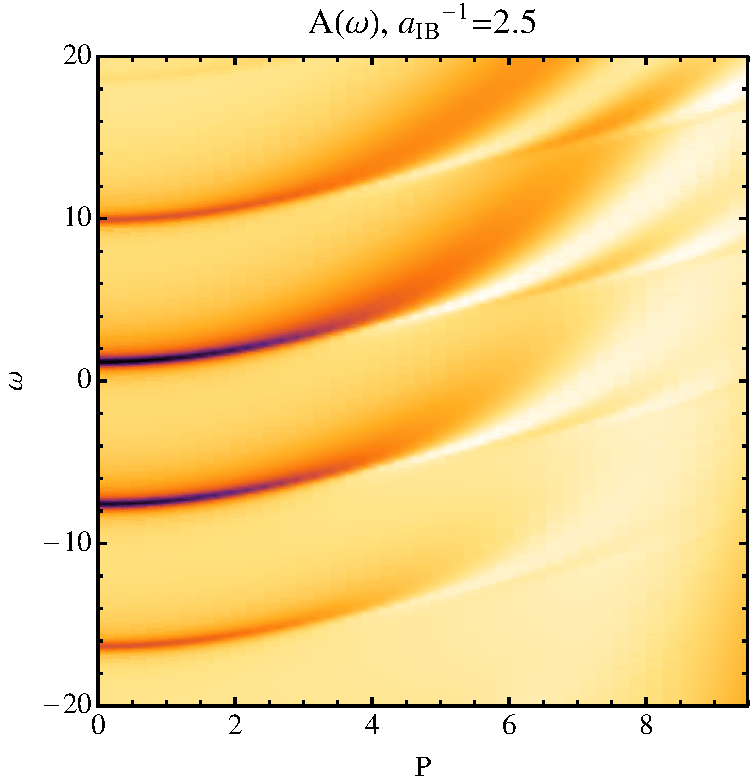
\includegraphics[clip,width=1\columnwidth]{figures/Spectral_func_aIB_2_5.pdf}
\caption{\label{fig:DynAttr} } 
\end{figure}


\subsection{Subsonic-supersonic transition}

%\subsection{Polaron formation}
%
%\begin{figure}[t]
%\centering{}%
%\begin{tabular}{c}
%\includegraphics[clip,width=1\columnwidth]{figures/quench_attractive_polaron}\tabularnewline
%\end{tabular}
%\caption{Dynamics of the polaron formation on the attractive side with $a_{IB}^{-1} = -5$ after the instantaneous quench of interactions. Initially impurity has momentum $P = 0.1,$(yellow), $0.85$(green), $0.9$(blue), $1$(red). Top and bottom panels show the dynamics of the number of phonons $N_\text{ph}$ and the momentum of the bosons $P_B$ (solid lines) and impurity $P_I$ (dashed lines) correspondingly. For the numerical calculations we use $\Lambda=20$.} 
%\label{fig:DynAttr}
%\end{figure}
%
%\begin{figure}[t]
%\centering{}%
%\begin{tabular}{c}
%\includegraphics[clip,width=1\columnwidth]{figures/quench_repulsive_polaron}\tabularnewline
%\end{tabular}
%\caption{Dynamics of the polaron formation on the repulsive side with $a_{IB}^{-1} = 4$ after the instantaneous quench of interactions. Initially impurity has momentum $P = 0.1,$(yellow), $1$(green), $2.5$(blue). Top and bottom panels show the dynamics of the number of phonons $N_\text{ph}$ and the momentum of the bosons $P_B$ (solid lines) and impurity $P_I$ (dashed lines) correspondingly. For the numerical calculations we use $\Lambda=20$.}
%\label{fig:DynRep}
%\end{figure}
%
%
%We study the formation of the polaron in real time following the instantaneous quench of the interactions from $g_\Lambda =0$ to some finite value.
%Depending on the finite value of the interaction we see two very distinct regimes.
%
%On the attractive side, $a_{IB}^{-1} < 0$, the number of phonons excited by the impurity grows monotonically after the quench  (see Fig.~\ref{fig:DynAttr}(a)).
%Initial momentum of the impurity increases the creation rate of the excitations. Fig.~\ref{fig:DynAttr}(b) shows the dynamics of the total bosons momentum $P_B$ as well as the impurity momentum $P_I = P- P_B$. 
%
%On the repulsive side, $a_{IB}^{-1} > 0$, the number of phonons excited by the impurity shows oscillatory behavior after the quench  (see Fig.~\ref{fig:DynRep}(a)). As for the attractive polaron larger initial momentum of the impurity only marginally increases the creation rate of the excitations (though we are looking at the weak coupling regime in the both cases).  The dynamics of the total bosons momentum $P_B$ and the impurity momentum $P_I = P- P_B$ show the same type of the oscillatory behavior as the total number of excitation. This is due to the formation of the bound states. Two subsystems, the impurity and the Bogoluibov excitations, exchange their momentum of the time scale characterized by the  frequency of the bound states.
%
%\ys{In the small $P$ limit show the polaron mass $M_p$ as a function of time. Is there any other definition of mass we can use for an arbitrary momentum?}


\subsection{(Anomalous) diffusion}
\ys{Calculate $x^2(t)$ and figure out if it is normal or anomalous diffusion.}

To calculate the


\section{Dynamics of the released impurity}
\ys{Derive some expressions for the properties of impurities in real time after being released from the trapping potential. }

Consider several trapping geometries
\subsection{Harmonic oscillator trap}

\subsection{Pancake geometry}

\section{Discussion with Misha}
TO DO LIST: 
\begin{enumerate}
\item  $Z$-factor is the same for $S(t)$ and $n_k$
\item Check $Z$-factor of a static problem and dynamic problem is the same.
\item $\bra{\Psi_\text{pol}} P_\text{imp} \ket{\Psi_\text{pol}} \neq  \lim_{t \rightarrow \inf }\bra{\Psi(t)} P_\text{imp} \ket{\Psi(t)} $
\item Check $n_\text{imp}^\text{pol} = \lim_{t\rightarrow \inf} n_\text{imp}(t)$
\end{enumerate}

\begin{figure}[t]
\centering{}%
\begin{tabular}{c}
\includegraphics[clip,width=1\columnwidth]{figures/Zdyn_Zstat}\tabularnewline
\end{tabular}
\caption{}
\label{fig:DynRep}
\end{figure}



%\section{Superconic impurity}

\bibliography{Polaron1}
\end{document}
